\chapter{Определение смысловой близости пары наборов ключевых слов} \label{chapt_tuple_similarity}
В данном разделе представлены разработанные автором настоящей работы алгоритмы выявления смысловой близости между двумя наборами ключевых слов.  Этот уровень определяет уровень близости пары объектов интеллектуальной системы, с которыми были ассоциированы данные наборы ключевых слов.
Семантическая близость между наборами ключевых слов определяется с использованием введенных в предыдущей главе методах определения семантической близости между парой ключевых слов.
В конце раздела представлены результаты тестовых испытаний программных реализаций алгоритмов, выводы о выполненной работе, а также предлагаются идеи для дальнейшего улучшения качества определения семантической близости наборов ключевых слов.

\section{Алгоритмы определения смысловой близости наборов ключевых слов}

Дано множество документов $D$ и множество ключевых слов $W$. Каждый элемент $d_i \in D$ представлен набором из $k_i$ ключевых слов из множества $W: d_i = (w_{i,1},w_{i,2},...,w_{i,ki})$. Необходимо разработать такую функцию близости $TupleSim : 2^W \times 2^W \rightarrow [0, 1]$, высокие значения которой означали бы высокий уровень смысловой близости между наборами и, следовательно, соответствующими документами системы. 

Также к разрабатываемой метрике предъявляются следующие требования:
\begin{itemize}
    \item программная реализация должна быть способна вычислять значения метрики в режиме реального времени. Значительные задержки между отправленным пользователем запросом и полученным ответом не могут быть слишком долгими, иначе использование такой системы будет трудновыполнимым;
    \item необходимо уметь посчитать близость в том числе и для тех наборов, слова которых не представлены в системе. Существенная доля поисковых запросов содержит слова, которые ранее не были заданы ни разу и, что более важно, не встречаются в описаниях к документам системы.
\end{itemize}


Основой для разрабатываемой функции определения близости являются методы с средства, введенные в предыдущей главе: таким образом, в качестве базовых  блоков определения близости наборов естественно положить идеи о близости между словами, из которых эти наборы состоят. Другими словами, $TupleSim(d_i, d_j) = TupleSim(WordSim(w_{i,1}, w_{j,1}), ... , WordSim(w_{i,ki}, w_{j,kj}))$. 

При определении функции $TupleSim$ были использованы следующие соображения:
\begin{itemize}
    \item как правило, если ключевое слово
\end{itemize}


\subsection{Алгоритм определения близости пары наборов, основанный на переборе всех пар ключевых слов}
Первая версия алгоритма определения семантической близости наборов ключевых слов представлена далее:
\begin{itemize}
    \item входные данные: пара наборов $d_i = (w_{i,1},w_{i,2},...,w_{i,ki}), d_j = (w_{j,1},w_{j,2},...,w_{j,kj})$;
    \item для каждой пары ключевых слов $w_{i,p}, w_{j,q}$ с индексами $p \in [1, k_i], q \in [1, k_j]$:
        \begin{itemize}
            \item рассчитывается признаковые характеристики, описанные в \ref{sec:features};
            \item посчитанный массив значений передается предобученной модели XGBoost, описанной в \ref{sec:model};
            \item происходит предсказание пословной близости моделью;
            \item результаты сохраняются в ячейке $(p, q)$ матрицы $m_{sim}$ размером $k_i, k_j$.
        \end{itemize}
    \item из каждой строки матрицы $m_{sim}$ выбирается наибольшее значение;
    \item по этим наибольшим значениям вычисляется среднее. Это среднее возвращается в качестве меры близости для пары рассматриваемых наборов.
\end{itemize}

Далее приведены примеры близких наборов ключевых слов, согласно описанной модели. При построении примеров рассматривались наборы, имеющие пустое пересечение по словам - такие примеры представляют существенно больший интерес:

\textbf{[мультиферроики, магнитные структуры, фазовые переходы, магнитоэлектрики, сильные магнитные поля]}\
-
\textbf{[мультиферроики, магнитные структуры, фазовые переходы, магнитоэлектрики, сильные магнитные поля]}\

\begin{tabularx}{16cm}{|X|X|X|}
        \hline
        Первый набор & Второй набор & Значение функции близости \\ \hline
        мультиферроики, магнитные структуры, фазовые переходы, магнитоэлектрики, сильные магнитные поля & магниторезонансная томография, гигантское комбинационное рассеяние, суперпарамагнетизм & 0.82 \\ \hline
        мембранные белки, молекулярное моделирование, фоточувствительные белки, ретиналь, молекулярная динамика, membrane proteins, molecular modeling, retinal, molecular dynamics, photosensitive proteins & малые белки теплового шока, универсальный белковый адаптер 14-3-3, фосфорилирование & 0.68 \\ \hline
        социальная теория, социальная философия, понятие общества, философия истории & идея, социальная практика, научно-технический прогресс, наука, парадигма & 0.57 \\ \hline
        мультиферроики, низкоразмерные и фрустрированные магнитные системы, термодинамические и резонансные свойства, зарядовое и орбитальное упорядочение & магниторезонансная томография, гигантское комбинационное рассеяние, суперпарамагнетизм & 0.8 \\ \hline

\end{tabularx}


\subsection{Оптимизированный алгоритм определения близости пары наборов}

Описанный подход определения близости пары наборов ключевых слов с полным перебором всех пар ключевых слов по экспертной оценке имеет высокий уровень качества. Однако, он имеет существенный недостаток. Этот недостаток заключается в быстродействии предложенной модели. 

Существует несколько мест алгоритма, главным образом влияющих на скорость выполнения вычисления близости. Первый момент заключается в подсчете попарных уровней близости между словами разных наборов. Эта процедура имеет асимптотическую сложность $O(mn)$, где $m$, $n$ - размеры наборов. Таким образом, для пары наборов необходимо посчитать 30-50 уровней близости между словами этих наборов.

Отмечается, что значение вычисленных функций близости можно сохранять и переиспользовать. Кроме того, наивная версия алгоритма опирается на факт необходимости вычисления уровней близостей для всех возможных пар. С другой стороны, кажется логичным следующее предположение: если для слова из первого набора уже найдено близкое слово из второго, то нет необходимости продолжать сравнивать это слово с другими словами второго набора. Например, если в одном наборе присутствует слово <<белок>>, а в другом слово <<протеин>>, то установив факт близости, можно остановиться и не вычислять близость слова <<белок>> до других слов другого набора (<<мембранные белки>>, <<молекулярное моделирование>>, <<фоточувствительные белки>>, <<ретиналь>>)

Следующим узким местом с точки зрения производительности является непосредственно вычисление функции близости, определенную в главе \ref{chapt_word_similarity}.  Для вычисления близости необходимо применить обученную модель из раздела \ref{sec:model}. В наивном варианте алгоритма, описанного в предыдущем разделе, функция применения модели выполняется для каждой пары рассматриваемых слов. Однако, более эффективным является применение модели сразу для всего множества рассматриваемых пар.

На более низком уровне сложность вычисления зависит от скорости вычисления признаков для пары ключевых слов, описанных в \ref{sec:features}. Естественно, что все необходимые графы хранятся в оперативной памяти, их загрузка и построение происходит единожды до вычисления функций близости. При этом вычисления различных графовых характеристик (таких как длины путей, степени абстрактностей вершин и другие) выполняется каждый раз для каждой пары ключевых слов. Это значительно замедляет процесс, поэтому была проведена оптимизация вычисления признаков, которая будет описана далее.

Исходя из соображений, описанных выше, алгоритм был оптимизирован при помощи следующих средств:
\begin{itemize}
    \item в качестве значения близости между одинаковыми словами $WordSim(w, w)$ автоматически ставится уровень близости 1. Как было показано в разделе \ref{sec:test_equal}, модель умеет правильно определять наивысший уровень близости между словом и им самим же. Поэтому нет необходимости просчитывать эти значения и если в наборах встретились одинаковые слова, то можно сразу положить их близость равной максимальному значению;
    \item если для слова уже найдено близкое, то поиск вычисление близости до других слов не происходит. В качестве порога выбрано значение 0.4;
    \item кеширование значения близости для самых частотных пар. Для этого ключевые слова упорядочиваются по уменьшению частоты встречаемости в системе. Далее предвычисляются близости между всеми парами из первой тысячи самых частотных слов. Все значения сохраняются и далее используются в качестве кеша. Кроме этого вычисляются все пары из первой тысячи и первыми $10000$ слов. Среди них в кеш кладутся те пары, значения близости между которыми превышает порог (выбрано значение 0.4);
    \item кеширование значений признаков. Для одиночных признаков, описанных в разделе \ref{sec:features}, имеется возможность предрассчитать и закешировать значения. Это возможно, поскольку одиночных признаков (то есть тех, которые посчитаны только по одной вершине, а не по паре) значительно меньше (линейное по количеству уникальных слов системы) и с легкостью помещается в оперативной памяти;
    \item применение модели машинного обучения происходит в момент, когда все признаки для всех необходимых пар посчитаны. Это позволяет оптимально использовать матричные операции при вычислении значений формулы.
\end{itemize}

Данные средства позволили уменьшить среднее время выполнения вычисления близости в 20 раз.

\subsection{Тестовые испытания}
Для проведения эксперимента были взяты данные по научным проектам из ИАС <<ИСТИНА>>. О каждом проекте известная следующая информация: 
\begin{itemize}
    \item название;
    \item название на английском языке (может отсутствовать).
    \item идентификационный номер проекта;
    \item короткое текстовое описание проекта (может отсуствовать);
    \item набор ключевых слов (может отсутствовать);
    \item руководители участники проекта (заданы идентификационными номерами, может отстутствовать);
    \item департамент проекта (задан идентификационными номерами, может отсутствовать).
\end{itemize}

Всего в наборе данных присутствует информация о $12350$ проектах. 

Для тестирования программной реализации было проведено два качественных эксперимента над рассмотренным набором данных. Помимо этого был проведен замер производительности. Рассмотренная в настоящей главе модель определения близости наборов сравнивается с классической мерой близости Жаккара для наборов и моделью Word2Vec, обученной на огромном объеме (12.9 млрд. словоупотреблений) в рамках проекта Russian Distributional Thesaurus. Близость наборов моделью Word2Vec вычислялась по следующему алгоритму:
\begin{itemize}
    \item для каждого слова каждого набора рассматривались его векторные представления моделью;
    \item векторное представление набора определяется как среднее по векторам входящим в него слов;
    \item вычисляется косинусное расстояние между векторами наборов - оно возвращается в качестве близости наборов ключевых слов.
\end{itemize}
        
Далее описывается процедура каждого из экспериментов и приводятся результаты тестирования. 

\subsubsection{Тестирование близости по департаментам}
Естественно предположить, что  внутри одного департамента, проекты не так сильно отличаются друг от друга и, следовательно, ключевые слова проектов одного департамента должны быть в среднем более похожи друг на друга, чем слова разных департаментов.

Исходя из этих рассуждений, был подготовлен тестовый набор данных. В качестве примеров близких по смыслу наборов ключевых были взяты пары наборов, проекты которых принадлежат одному департаменту. Для каждого набора $W$, для которого определены положительные примеры $\overline{W}_{1}, ... \overline{W}_{k}$, случайным образом из множества проектов других департаментов выбирается 1000 проектов. Наборы $\hat{W_1}, ..., \hat{W}_{1000}$, соответсвующие этим проектам, объявляются семантически непохожими на набор $W$. Таким образом, для набора $W$ присутствует $k$ наборов, объявленных похожими по смыслу к $W$, и $1000$ наборов, объявленных непохожими.

Далее для каждого набора $W$ моделями $TupleSim$, $Word2Vec$ и  $Jaccard$ вычисляются меры близости. Но основе правильных ответов и ответов, определенных моделями, для каждого из подходов подсчитывается метрика $ROC-AUC$. Значение этой метрики усредняется по всем $W$.

Результаты тестирования приведены в следующей далее таблице \ref{tbl:tuple_test}:

Отмечается, что абсолютные значения в данном эксперименте не играют существенной роли: что набрать стопроцентный результат и даже близкий к нему не представляется возможным в силу построения тестирущего множества. Дело в том, что в действительности проекты одного департамента не обязаны быть строго похожими друг на друга. Напротив, многие из них могут сильно различаться, но согласно эксперименту, в этом случае они все равно будут объявлены как близкие и если модели факт близости не установят, то значение метрики уменьшится. 

Однако, связь между близостью наборов и принадлежностью их к одному департаменту присутствует. Разработанная автором настоящей диссертации модель лучше других известных моделей установила эту связь, что является показателем ее качества.

\subsubsection{Тестирование наборов с общими словами}

Данный эксперимент аналогичен предыдущему, но вместо факта принадлежности пары проектов одному департаменту используется факт существования общего ключевого слова у ключевых наборов двух проектов. Предполагается, что вероятность семантической близости пары наборов, имеющих общее слово, выше, чем случайной пары наборов. Более сильное предположение, что даже если удалить это общее слово, все равно близость между такими наборами должна быть в среднем выше, чем у случайных.

Множества $\overline{W}_{1}, ... \overline{W}_{k}$ и $\hat{W_1}, ..., \hat{W}_{1000}$ собирались таким же способом, как в предыдущем эксперименте. Результаты тестовых испытаний приведены в таблице \ref{tbl:tuple_test}

Отмечается, что и в этом испытании разработанная модель показала лучший результат. Важно также отметить, что модель $Jaccard$ отстает более значительно от двух других. Причиной этому является то, что удаление общего слова в рассматриваемых парах в подавляющем большинстве случаев (порядка 80\%) означает, что больше общих слов в наборах не осталось. По определению меры Жаккара, близость для таких наборов будет равна нулю. А это значит, что у таких примеров нет возможности сделать метрику качества выше 0.5.

\subsubsection{Тестирование производительности}
Для тестирования было замерено время подсчета функция близости для трех моделей на обоих качественных экспериментах. Результаты также приведены в таблице \ref{tbl:tuple_test}. Стоит отметить, что модель $Word2Vec$ обучена на огромных объемах данных. Время обучения такой модели требует недель или месяцев процессорного времени. Однако это дает возможность более эффективно использовать обученные векторные представления и быстро подсчитывать функцию близости. Модель $Jaccard$ способна подсчитывать близость быстро засчет свой простоты. Несмотря на это, разработанная модель $TupleSim$ способна показывать лучшее качество, с относительно небольшим отставанием по времени.

\begin{table}
\begin{tabularx}{16cm}{|X|X|X|X|} 
        \hline
        Модель & Тип тестирования & Метрика ROC-AUC &  Время подсчета в сек. \\ \hline
        Jaccard & Департаменты &0.564 & 8 \\ \hline
        Word2Vec & Департаменты &0.672 & 12 \\ \hline
        \textbf{TupleSim} & Департаменты & \textbf{0.692} & 15 \\ \hline
        Jaccard & Общее слово & 0.601 & 3 \\ \hline
        Word2Vec & Общее слово & 0.720 & 4 \\ \hline
        \textbf{TupleSim} & Общее слово& \textbf{0.764} & 8 \\ \hline
\end{tabularx}

\caption{Результаты тестирования} \label{tbl:tuple_test}
\end{table}




%\section{Алгоритмы определения смысловой близости коротких предложений}
%\section{Методы кластеризации наборов ключевых слов}
\section{Определение тематической направленности набора ключевых слов} \label{theme_tags}
В данном разделе ставится задача определения тематической направленности набора ключевых слов и дается разработанное автором настоящей диссертации решение.

Пусть, как и ранее, дано множество документов $D$ и множество ключевых слов $W$. Каждый элемент $d_i \in D$ представлен набором из $k_i$ ключевых слов из множества $W: di = (w_{i,1},w_{i,2},...,w_{i,ki})$. Необходимо разработать методы определения тематики для каждого документа коллекции. Под тематикой следует понимать название некоторой области знаний, дисциплины, специальности или направления. Определив такое слово для документа, можно с высокой вероятностью сказать о чем этот документ. Тематическое ключевое слово - это такое ключевое слово из $W$, которое может являться тематикой документа. Таким образом, необходимо из множества ключевых слов $W$ выделить подмножество $T \subset W$ тематических ключевых слов и для каждого документа из коллекции определить соответствующее ему множество тематических ключевых слов, т.е. определить отображение $t : D \rightarrow 2^T$ . Отметим, что принадлежность ключевых слова к тематике зависит от набора документов.

В множестве ключевых слов, которые приписаны документам из некоторой коллекции, можно выделить <<тематические ключевые слова>> - ключевые слова, семантическое значение которых является названием некоторого <<широкого>> направления. Примерами таких ключевых слов могут быть: <<динамика>>, <<статистика>>, <<право>>, <<численные методы>>. Выделение таких слов из набора является простой задачей для человека, но очень сложной для машины. В настоящем разделе описывается алгоритм, определяющий тематику набора ключевых слов, а также приводятся результаты его работы на реальных данных. Предложенные алгоритмы опираются на понятие абстрактности ключевого слова, а также на алгоритм её определения.


\subsection{Описание алгоритма выбора тематики набора}
После того, как сформировано множество тематических ключевых слов, появляется возможность определить тематику целого набора. Для этого необходимо взять ключевых слово с наибольшем уровнем абстрактности. Описание методов определения уровней абстрактности приведено в \ref{abstr} Если такое ключевое слово лежит в множестве тематических, то можно выдать его в качестве ответа. В противном случае, необходимо найти ближайшее тематическое ключевое слово из графа ключевых слов. Для этого сначала берутся соседи исходной вершины. Полученное множество просматривается на наличие в нем тематических ключевых слов. Если такие ключевые слова присутствуют, то все они возвращаются в качестве ответа (таким образом для набора выбирается несколько возможных тем), иначе просматриваются соседи соседей и т.д. В некоторых случаях определить тематическую направленность не представляется возможным. Очевидно, это происходит тогда, когда в компоненте связности самого абстрактного ключевые слова в наборе не присутствует ни одного тематического ключевого слова.  Отметим, что учитывается тот факт, что если расстояние между парой ключевых слов в графе велико, то нельзя выделить какую-либо семантическую связь между этими ключевыми словами. Также заметим, что если радиус круга соседей будет слишком велик, то очень вероятно, что в множество тематических слов попадёт слишком много слов. Для решения этих задач введён параметр r, который показывает максимальное возможное расстояние в графе между исходным ключевым словом и ближайшем найденным тематическим. Если в радиусе $r$ тематическое ключевое слово найти не удалось, то тема набора не определена. В программной реализации алгоритма значение $r$ равно 2.

\subsection{Тестовые испытания}
Тестирование программное реализации алгоритма проводилось на данных, описанных в разделе \ref{abstr_test}. Некоторые из результатов приведены в таблице \ref{tbl:theme_table_1}

\begin{figure}[ht]
  \begin{minipage}[ht]{1.0\linewidth}\centering
    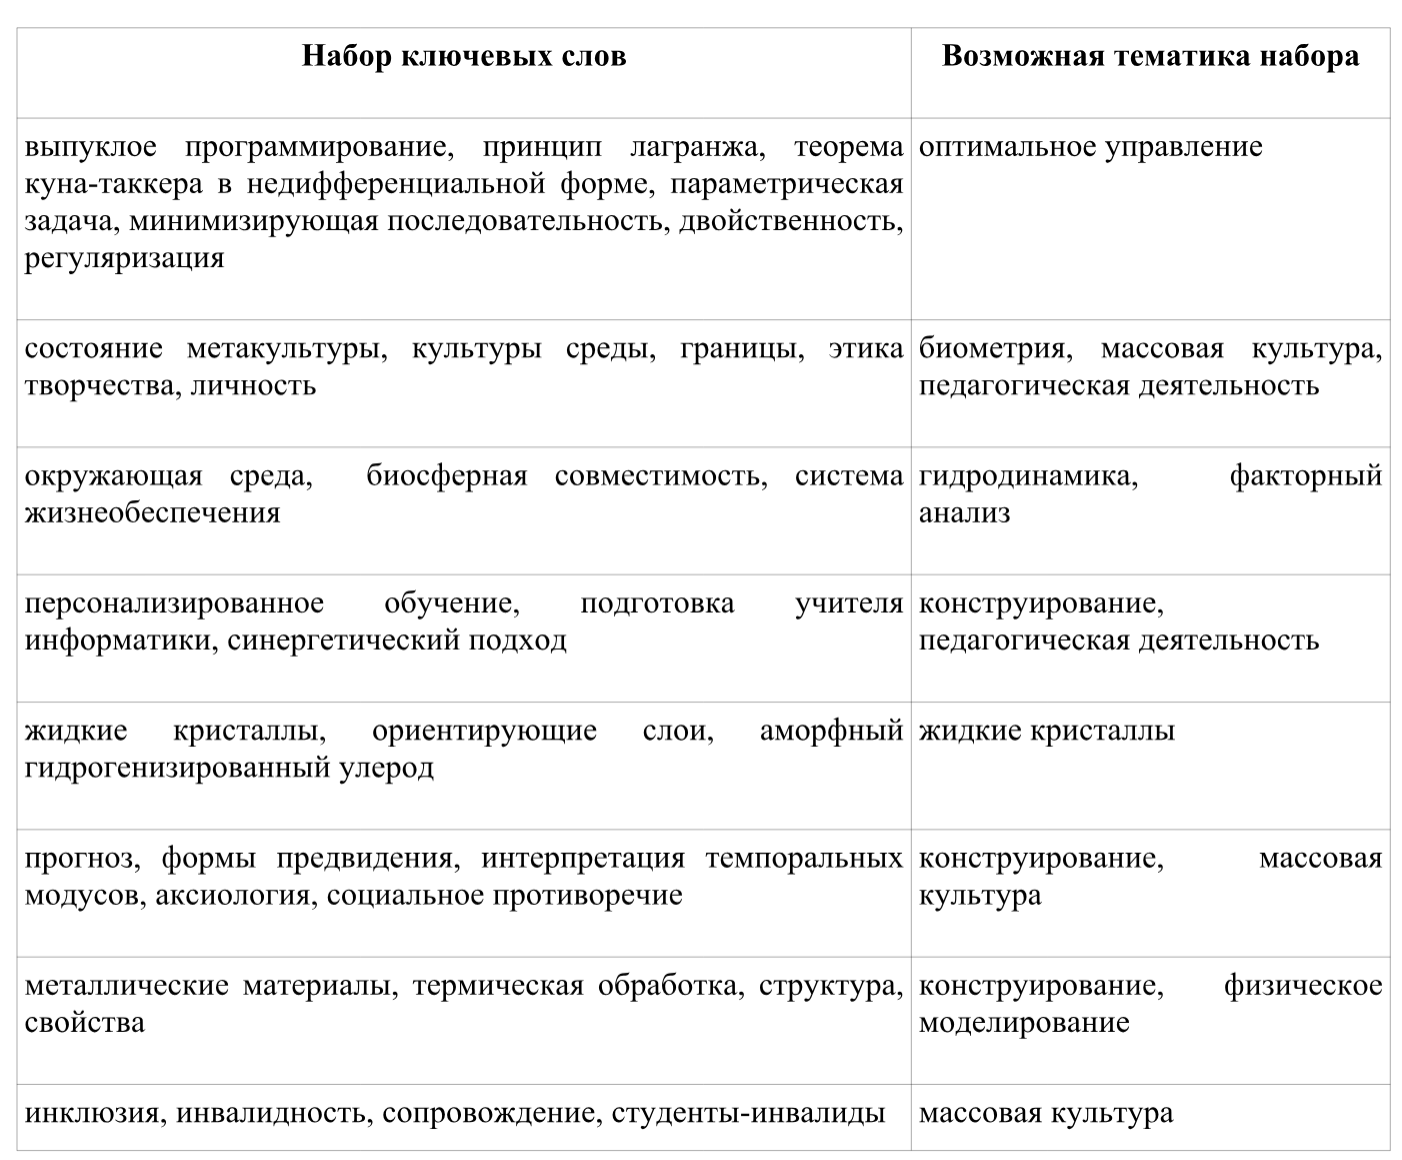
\includegraphics[width=1.0\linewidth]{Dissertation/pics/theme_table_1}
  \end{minipage}
  \label{tbl:theme_table_1}
\end{figure}

\begin{figure}[ht]
  \begin{minipage}[ht]{1.0\linewidth}\centering
    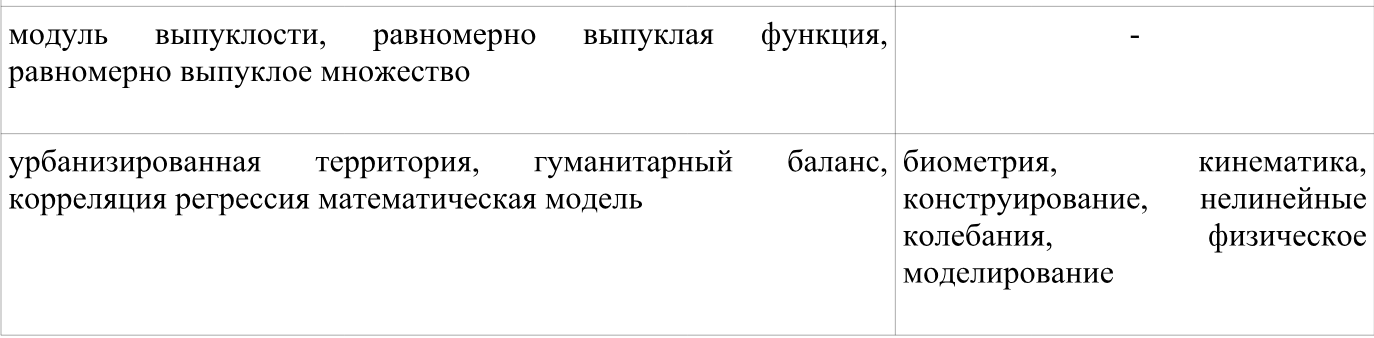
\includegraphics[width=1.0\linewidth]{Dissertation/pics/theme_table_2}
    \caption{Наборы и предсказанные им тематические направления}
  \end{minipage}
  \label{tbl:theme_table_2}
\end{figure}

В первом примере показано верное определение тематики. При этом можно заметить отсутствие тематического ключевого слова в исходном наборе. Последние два примера демонстрируют случаи, когда тематическое ключевое слово не определено или определено слишком большое число таких слов.

В целом, следует отметить, что алгоритм допускает достаточно много ошибок. Очень часто ошибка возникают на наборах, состоящих только из редких слов-терминов. Причина в том, что слова в подобных наборах не соединены напрямую с тематическими, а увеличение пути сильно уменьшает качество результатов. Не определяется тематика и у тех наборов, ключевые слова которых попали в малые компоненты связности без тематических ключевы слов. Однако основная трудность - это накопление ошибок разных алгоритмов. Сначала слово ошибочно получило высокий уровень абстрактности, затем попал в список тематических и, в итоге, неправильно определена тематика набора.

Несмотря на отмеченные недостатки, предложенный подход потенциально может быть улучшен. Для этого можно использовать все ключевые слова из набора для определения тематики, проверять абстрактности вершин на пути от данного ключевого слова к тематическому и использовать многие другие эвристики. Однако уже сейчас можно констатировать, что алгоритм способен с некоторой точностью решать поставленную задачу. 

%\begin{table} [htbp]% Пример записи таблицы с номером, но без отображаемого наименования
%	\centering
%	\parbox{18cm}{% чтобы лучше смотрелось, подбирается самостоятельно
%        \captiondelim{}% должен стоять до самого пустого caption
%        \caption{}%
%        \label{tbl:test1}%
%        \begin{SingleSpace}
%    	\begin{tabular}{ | c | c |}
%    	\hline
%    	выпуклое программирование, принцип лагранжа, \\
%        теорема куна-таккера в недифференциальной форме, \\
%        параметрическая задача, \\
%        минимизирующая последовательность, двойственность\\
%        , регуляризация & оптимальное \\ управление \\ \hline
%    	\end{tabular}%
%    	\end{SingleSpace}
%	}
%\end{table}

\section{Решение задачи поиска экспертов} \label{expert_search_tuplesim}
\subsection{Определение близости наборов для решения задачи поиска экспертов}
В качестве меры близости пары наборов ключевых слов автором предлагается следующая формула:
$$ TupleSim_{expert}(X,Y) = \frac{\sum_{i=1}^{|X|}\sum_{j=1}^{|Y|}WordSim_{expert}(X_i, Y_j)}{|X \bigcup Y|}, $$

где $|\cdot|$ ­ количество слов в наборе, $X_i$, $Y_j$ ­ $i$­ое и $j$­ое ключевые слова наборов $X$, $Y$ соответственно. $WordSim_{expert}$ - мера близости, введенная в \ref{expert_search_wordsim}. Числитель этой формулы аккумулирует близость всех пар слов из разных наборов. Если положить $WordSim_{expert}(x, y) = \mathbbm{1}x=y$, то числитель будет равен числу общих ключевых слов, что приведет к более простой модели вычисления близости по мере Жаккара. Без нормировки длинные пары наборов были бы сильнее похожи друг на друга, чем короткие пары.

%\section{Выводы}
%...
